\chapter{Data}
\label{sec:data}


In this section I talk about different datasets word2doc uses. More specifically, I talk about training and evaluation datasets
as well as pre-trained models that word2doc uses, and how these models might perform even better when custom trained.

\section{Training Data}

First, I will talk about how word2doc's training data is generated. I will talk a bit about overfitting and problems related to
it, and then I delve into the details of generating the training data itself.

\subsection{Overfitting}
\label{data:overfitting}

As mentioned before, word2doc operates on the entire English Wikipedia corpus, and is thus trained on the entire Wikipedia corpus,
similar to the way word embeddings are trained on their own corpus. This is not an issue from an overfitting perspective, because
we want overfitting to occur, as explained in section \ref{theory:training}.

However, it is possible that word2doc memorizes document-title pairs instead of learning the semantic meaning behind each. What I
mean is that word2doc could learn to match query "football" with document "football", not because it understands that
both share a similar context, but because they mostly only occur together. When "soccer" is then used instead of "football", the
net might not be able to identify that football and soccer share a similar meaning, because it only learned the title document
associations which is pointless anyway (we know what title belongs to what document).

In word embeddings this problem solves itself, because the context a word appears in always varies (section \ref{theory:embb}). For
example, the word "football" will occur together with so many different words, that there is little risk of building a one-to-one
connection like described above. However, since word2doc is trained with Wikipedia document-title pairs, it is inherently so that
a query (the title) is very likely to occur most often with its own document. In other words, documents do not have multiple titles,
and titles do not have multiple documents, and this is a problem.

To counter this problem, I perform data augmentation. The title is dissected into important keywords (if the title is
long enough) and the six most important keywords of the first paragraph of each Wikipedia document are extracted using rake
\citep{rake}, a keyword extraction tool. More specifically, I take the first two keywords from the very first sentence of a
document, which is usually the topic sentence and thus it summarizes the document well. I then take four keywords from the remaining
paragraph, which is the introduction paragraph. It should be noted, that not every query receives six keywords. Sometimes the first
paragraph is not long enough, resulting in fewer than six keywords extracted. Thus, not every query has exactly six keywords.

The first (introduction) paragraph of a Wikipedia article is almost always a brief summary of the article itself, which is a nice
feature I am exploiting. That means the six most important keywords of the first paragraph are likely to be
six important keywords describing the document. Using six keywords instead of two or three means that the later keywords fit the
document less and less and thus they are more likely to also occur in different documents. Each of these six keywords is then
paired with the target document, which remains the same. For example, let's say the "Artificial Neural Network" document (ID: 324923)
has the following 5 keywords: neural, network, brain, programming and label. The data would be augmented with the following pairs:
(neural, 324923), (network, 324923), (brain, 324923), (programming, 324923) and (label, 324923). Each pair will now be treated
independently of each other, as its own separate data point.

If each individual keyword is paired with the original document in the way it is explained above, we should have conditions closer
to those of word embeddings. Queries now share multiple documents since the extracted keywords are not unique to one document, and
documents can share multiple queries. Ultimately, we will have gone from a one-to-one mapping between queries and documents to
an n-to-n mapping. I call these keywords \textit{pivots}, not to be confused with pivots in word2vec \citep{word2vec}. I call them
pivots because the keywords pivot around the original document. When a sentence embedding is applied to them, I call
them \textit{pivot embeddings}.

Thus, my claim from section \ref{theory:training} that word2doc is only trained by using document titles as queries and the documents
themselves as labels is not entirely accurate. For each document there are up to seven different data points. Of course augmented
data points share the same context documents, since they all share the same label (the target document).

\subsection{Wikipedia Dump}

To obtain the English Wikipedia corpus, I downloaded a Wikipedia dump and processed it with Giuseppe Attardi's Wikiextractor tool
\footnote{\url{https://github.com/attardi/wikiextractor}}. The tool extracts text from the dump, along with metadata like the url
and the title and saves the content to many JSON files, where it is then saved into a database to be processed by word2doc.

\subsection{Generating Training Data}

Once the entire English Wikipedia corpus is pre-processed, word2doc iterates through every single document to generate the
necessary data for the neural network. That means for every document, context documents are calculated, and for every query, a
query embedding is created. To be more efficient, the data is split into 100 bins of equal size, with 10 bins being processed at a
time through a SLURM queue. Table \ref{tbl:train-data} illustrates what a data point in the training data looks like.

\begin{table}[H]
  \centering
  \begin{tabular}{|p{3cm}|p{9cm}|}
    \hline
    \multicolumn{2}{|c|}{Training Dataset Excerpt} \\
    \hline
    Document title&Hand crafted query\\
    \hline
    \hline
    doc\_index:&1198816\\
    doc\_title:&Commonwealth Railways\\
    &\\
    pivot\_embeddings&[[ 0.02357988,  0.01399379, ..., -0.03814263, -0.02892261],\\
    &[ 0.05076515, -0.08939897, ..., -0.03814263, -0.02892261],\\
    &[ 0.1395378 ,  0.05702531, ..., -0.02987907, -0.02892261],\\
    &[ 0.0112771 , -0.08939897, ..., -0.03814263, -0.02892261],\\
    &[ 0.00092854,  0.00179368, ..., -0.03814263, -0.02830232]]\\
    &\\
    doc\_window&[2678437, 2312586, 1198826, 5040959, 1198834, 1198831, 2198060, 1198816, 1198827, 1198817]\\
    \hline
  \end{tabular}
  \caption{Training Dataset Excerpt}
  \label{tbl:train-data}
\end{table}

Looking at Table  \ref{tbl:train-data}, the document index is the ID of the Wikipedia article and serves as a label for the
neural network. The pivot embeddings are all the pivots processed into 4096 long sentence embedding vectors. That means, for
the document "Commonwealth Railways" there were 4
pivots plus the original title which is at position 0 of the array, resulting in a total of 5 pivot embeddings. And last but not
least, the document window which are the context documents for \textit{Commonwealth Railways}. This data is fed to the neural
network, where each pivot embedding is extracted, paired with the label (document ID) and context documents, and added as an
individual data point.

When this pre-processing step is complete with all 5,316,954 Wikipedia articles, the result is 100 bins, each with a size between
five and six Gigabytes. In total, around 600 GB of data is generated this way, and then processes by the neural network.


\section{Validation Data}
\label{data:eval}

Testing the performance of word2doc is not trivial (explained in section \ref{exp:eval}), and to do a better job, I generated two
evaluation datasets consisting of 200 and 400 hand crafted data points each. In this section I talk about how I created these data
points, and then I briefly mention how they are used in word2doc. The dataset of size 200 is called \textit{W2D-VD-200} for
word2doc validation data 200, and the dataset of size 400 is called \textit{W2D-VD-400}.

To create these data points by hand, I built a testing module for word2doc (\textit{word2doc-net-test.py}) that presents me
with a random document from a sub-selection of 5000 documents. These data points were randomly sampled from the full dataset.
For each random document, I am presented with the document title and the introduction paragraph, and from those I create a query
by hand. This hand made query is then added to the evaluation dataset as an individual data point. An excerpt of this dataset is
shown in Table \ref{tbl:eval-data}.

\begin{table}
  \centering
  \begin{tabular}{|p{1cm}|p{6cm}|p{6cm}|}
    \hline
    \multicolumn{3}{|c|}{Evaluation Dataset Excerpt} \\
    \hline
    No.&Document title&Hand crafted query\\
    \hline
    \hline
    1.&Strike Back: Project Dawn&project dawn tv series\\
    2.&National Operational Intelligence Watch Officer's Network&NOIWON secure conference call\\
    3.&RARRES1&Retinoic acid receptor responder protein 1\\
    4.&Medicine 8&Medicine eight\\
    5.&Nigel Parry&new york photographer parry\\
    6.&Guigues VIII of Viennois&guigues ofnvienne\\
    \hline
  \end{tabular}
  \caption{Evaluation Dataset Excerpt}
  \label{tbl:eval-data}
\end{table}

Most of the time the query is a brief description of the document, similar to what I would type into a Google search. Since I
created these queries myself, they are subject to a certain human bias, meaning I would not be surprised if I, without really
knowing it, constructed the queries in a way that I deem them more likely to succeed, since I ultimately want them to succeed. To
counter this, and to also make the test more realistic, I included tougher data points as well. More specifically, the
model has to deal with typos (number 6.), it has to understand abbreviations (number 2.), and it has to turn numbers into their written
form (number 3.). It did this surprisingly well, suggesting the model did learn something, but more to that in section
\ref{results}. The exact composition of each dataset is found in Figure \ref{fig:dataset-comp}.

\begin{figure}
  \begin{center}
    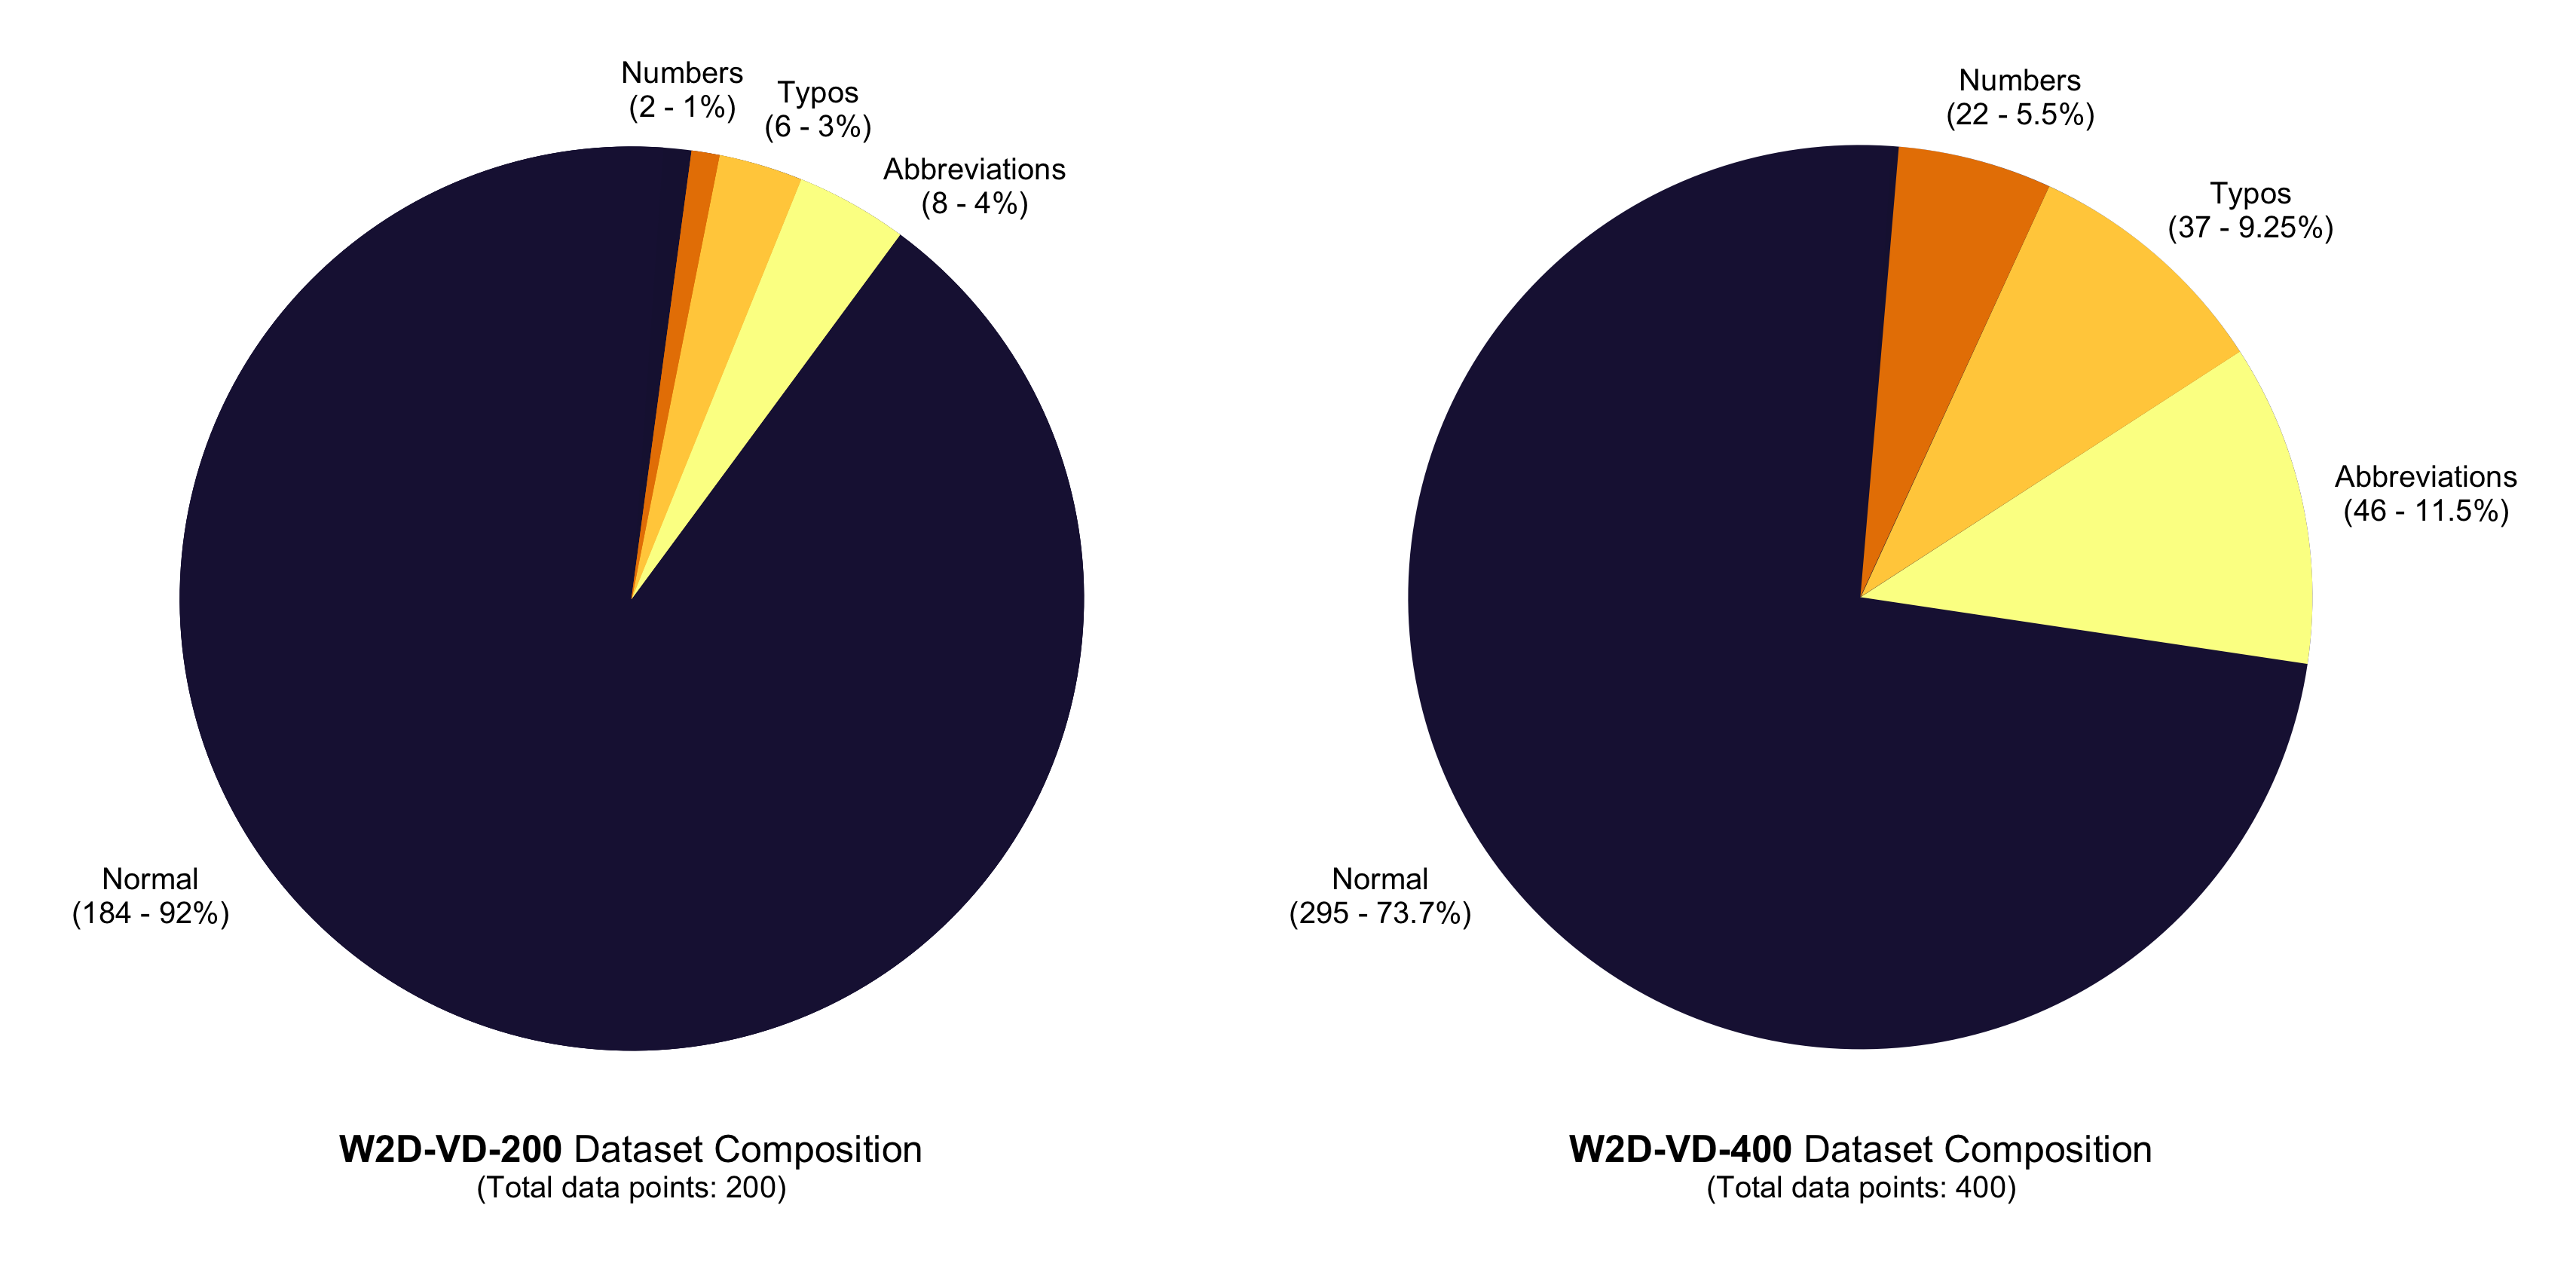
\includegraphics[scale=0.12]{test-data-split.png}
  \end{center}
  \caption{Composition of W2D-VD-200 and W2D-VD-400 datasets.}
  \label{fig:dataset-comp}
\end{figure}

In Figure \ref{fig:dataset-comp}, "normal" refers to data points that have not been manipulated in any way. The "abbreviation"
category is a broader term for cases in which one of the documents is refereed to by an alternative title. This can be a typical
abbreviation, but it can also be a nickname or a title in another language. The abbreviation category is testing the net's ability
to learn multiple terms for the same concept. The typos category is self-evident, it contains intentionally created typos. Finally,
it should be noted that W2D-VD-200 is a subset of W2D-VD-400 with more emphasis on "normal" data points. W2D-VD-200 is used in
section \ref{exp:dl} to measure performance of different word2doc models, and W2D-VD-400 is used to evaluated word2doc in section
\ref{results}.


\section{InferSent}

At last, I will talk about the trained InferSent model used in word2doc. I did not train it myself, instead I used
Facebook's pre-trained model, trained on what Facebook called AllNLI, made up of the SNLI and MultiNLI datasets. I already talked
about SNLI in section \ref{theory:inf}, and MultiNLI is the NYU's Multi-Genre NLI corpus, similar in structure to the SNLI corpus
from Table \ref{tbl:snli}. Both datasets are used because a significant boost in performance was observed using both datasets,
compared to just SNLI \citep{infersent}.

The authors of InferSent note in their conclusion, that this work only scratches the surface and that they believe with more
complete datasets significant improvements can be made to the quality of sentence embeddings. In the context of word2doc, this
could mean that using more complete datasets, or domain specific datasets (if word2doc were to run in only a certain domain)
could potentially improve final results.


\subsection{GloVe}

InferSent uses GloVe vectors during training. GloVe stands for Global Vectors for Word Representation, and is a collection of
pre-trained word vectors part of Stanford NLP \citep{glove}. Through GloVe vectors, InferSent uses a vocabulary consisting
of over 2.2 million of the most common english words to generate sentence embeddings. Instead of using pre-trained GloVe vectors,
it could be an option to train word embeddings on vocabulary most likely to occur in word2doc's domain, if one were
to use word2doc on a specific domain. Like I mentioned in the introduction, \citet{diaz2016} claim that global embeddings like
pre-trained GloVe vectors are underperformed by locally trained embeddings. However, GloVe vectors are very established and
since they are very general and since the Wikipedia corpus is also very general, they are probably a pretty good match nonetheless.

More specifically, InferSent uses the \textit{glove.840B.300d.txt} collection, a collection of pre-trained word vectors based on
a Common Crawl \footnote{\url{http://commoncrawl.org/}} data. Common Crawl builds all kinds of datasets by crawling the internet.
The Common Crawl GloVe model InferSent uses has 840 byte tokens, a vocabulary size of 2.2 million, it is cased, and has vectors
of dimension 300.

If you go on the GloVe website and look at the models available, you might notice that there is actually a model available
specifically trained on a 2014 Wikipedia dump. However, it has only has a vocabulary of size 400,000 and thus is much smaller
than the Common Crawl dataset which makes it less suited for the task. Ultimately a much larger vocabulary is better,
because it means the chance of encountering an OOV word is much smaller. InferSent can still process OOV words, as I
explained in section \ref{theory:inf} but it does a better job if the word is included in the pre-trained vocabulary.
